% This file is part of GUFI, which is part of MarFS, which is released
% under the BSD license.
%
%
% Copyright (c) 2017, Los Alamos National Security (LANS), LLC
% All rights reserved.
%
% Redistribution and use in source and binary forms, with or without modification,
% are permitted provided that the following conditions are met:
%
% 1. Redistributions of source code must retain the above copyright notice, this
% list of conditions and the following disclaimer.
%
% 2. Redistributions in binary form must reproduce the above copyright notice,
% this list of conditions and the following disclaimer in the documentation and/or
% other materials provided with the distribution.
%
% 3. Neither the name of the copyright holder nor the names of its contributors
% may be used to endorse or promote products derived from this software without
% specific prior written permission.
%
% THIS SOFTWARE IS PROVIDED BY THE COPYRIGHT HOLDERS AND CONTRIBUTORS "AS IS" AND
% ANY EXPRESS OR IMPLIED WARRANTIES, INCLUDING, BUT NOT LIMITED TO, THE IMPLIED
% WARRANTIES OF MERCHANTABILITY AND FITNESS FOR A PARTICULAR PURPOSE ARE DISCLAIMED.
% IN NO EVENT SHALL THE COPYRIGHT HOLDER OR CONTRIBUTORS BE LIABLE FOR ANY DIRECT,
% INDIRECT, INCIDENTAL, SPECIAL, EXEMPLARY, OR CONSEQUENTIAL DAMAGES (INCLUDING,
% BUT NOT LIMITED TO, PROCUREMENT OF SUBSTITUTE GOODS OR SERVICES; LOSS OF USE,
% DATA, OR PROFITS; OR BUSINESS INTERRUPTION) HOWEVER CAUSED AND ON ANY THEORY OF
% LIABILITY, WHETHER IN CONTRACT, STRICT LIABILITY, OR TORT (INCLUDING NEGLIGENCE
% OR OTHERWISE) ARISING IN ANY WAY OUT OF THE USE OF THIS SOFTWARE, EVEN IF
% ADVISED OF THE POSSIBILITY OF SUCH DAMAGE.
%
%
% From Los Alamos National Security, LLC:
% LA-CC-15-039
%
% Copyright (c) 2017, Los Alamos National Security, LLC All rights reserved.
% Copyright 2017. Los Alamos National Security, LLC. This software was produced
% under U.S. Government contract DE-AC52-06NA25396 for Los Alamos National
% Laboratory (LANL), which is operated by Los Alamos National Security, LLC for
% the U.S. Department of Energy. The U.S. Government has rights to use,
% reproduce, and distribute this software.  NEITHER THE GOVERNMENT NOR LOS
% ALAMOS NATIONAL SECURITY, LLC MAKES ANY WARRANTY, EXPRESS OR IMPLIED, OR
% ASSUMES ANY LIABILITY FOR THE USE OF THIS SOFTWARE.  If software is
% modified to produce derivative works, such modified software should be
% clearly marked, so as not to confuse it with the version available from
% LANL.
%
% THIS SOFTWARE IS PROVIDED BY LOS ALAMOS NATIONAL SECURITY, LLC AND CONTRIBUTORS
% "AS IS" AND ANY EXPRESS OR IMPLIED WARRANTIES, INCLUDING, BUT NOT LIMITED TO,
% THE IMPLIED WARRANTIES OF MERCHANTABILITY AND FITNESS FOR A PARTICULAR PURPOSE
% ARE DISCLAIMED. IN NO EVENT SHALL LOS ALAMOS NATIONAL SECURITY, LLC OR
% CONTRIBUTORS BE LIABLE FOR ANY DIRECT, INDIRECT, INCIDENTAL, SPECIAL,
% EXEMPLARY, OR CONSEQUENTIAL DAMAGES (INCLUDING, BUT NOT LIMITED TO, PROCUREMENT
% OF SUBSTITUTE GOODS OR SERVICES; LOSS OF USE, DATA, OR PROFITS; OR BUSINESS
% INTERRUPTION) HOWEVER CAUSED AND ON ANY THEORY OF LIABILITY, WHETHER IN
% CONTRACT, STRICT LIABILITY, OR TORT (INCLUDING NEGLIGENCE OR OTHERWISE) ARISING
% IN ANY WAY OUT OF THE USE OF THIS SOFTWARE, EVEN IF ADVISED OF THE POSSIBILITY
% OF SUCH DAMAGE.



\section{gufi\_query}

\subsection{Outline}

\texttt{gufi\_query} is used in order to query information from the generated databases that include all of the information about the indexed root directory and its sub-directories while also taking into account permissions
\subsection{Flags}

\begin{table} [h]
\centering
\begin{tabular}{l|p{6cm}}
Flag & Functionality \\\hline
-h & help\\
\hline
-H & show assigned input values (debugging)\\
\hline
-E \textless SQL ent\textgreater & SQL for entries table \\
\hline
-S \textless SQL sum\textgreater (will be read first) & SQL for summary table\\
\hline
-T \textless SQL tsum\textgreater & SQL for tree-summary table\\
\hline
-a & AND/OR (SQL query combination)\\
\hline
-n \textless threads\textgreater & number of threads\\
\hline
-j & print the information in terse form\\
\hline
-o \textless out\_fname\textgreater & output file (one-per thread, with thread-id suffix) implies -e 1\\
\hline
-d \textless delim\textgreater & one char delimiter \\
\hline
-O \textless out\_DB\textgreater & output DB, implies -e 1 \\
\hline
-I \textless SQL\_init\textgreater & SQL init \\
\hline
-F \textless SQL\_fin\textgreater & SQL cleanup \\
\hline
-y \textless min-level\textgreater & minimum level to descend to \\
\hline
-z \textless max-level\textgreater & maximum level to descend to\\
\hline
-J \textless SQL\_interm\textgreater & SQL for intermediate results (no default: recommend using "SELECT * FROM entries") \\
\hline
-K \textless create aggregate\textgreater & SQL to create the final aggregation table (if not specified, -I will be used)\\
\hline
-G \textless SQL\_aggregate\textgreater & SQL for aggregated results (no default: recommend using "SELECT * FROM entries")\\
\hline
-e \textless 0 or 1\textgreater & 0 for aggregate, 1 for print without aggregating (implied by -o and -O)\\
\hline
-m & Keep mtime and atime same on the database files \\
\hline
-B \textless buffer size\textgreater & size of each thread's output buffer in bytes \\
\hline
-w & open the database files in read-write mode instead of read only mode
\end{tabular}
\caption{\label{tab:widgets}gufi\_query Flags and Arguments}
\end{table}

\clearpage

\subsection{Example Calls}

\texttt{gufi\_query -S "SELECT * FROM summary" ~/directory\_of\_root\_index}
\\
\texttt{gufi\_query -E "SELECT * FROM pentries" ~/directory\_of\_root\_index}

\subsection{Visualizing the Workflow}
\begin{figure} [h]
\centering
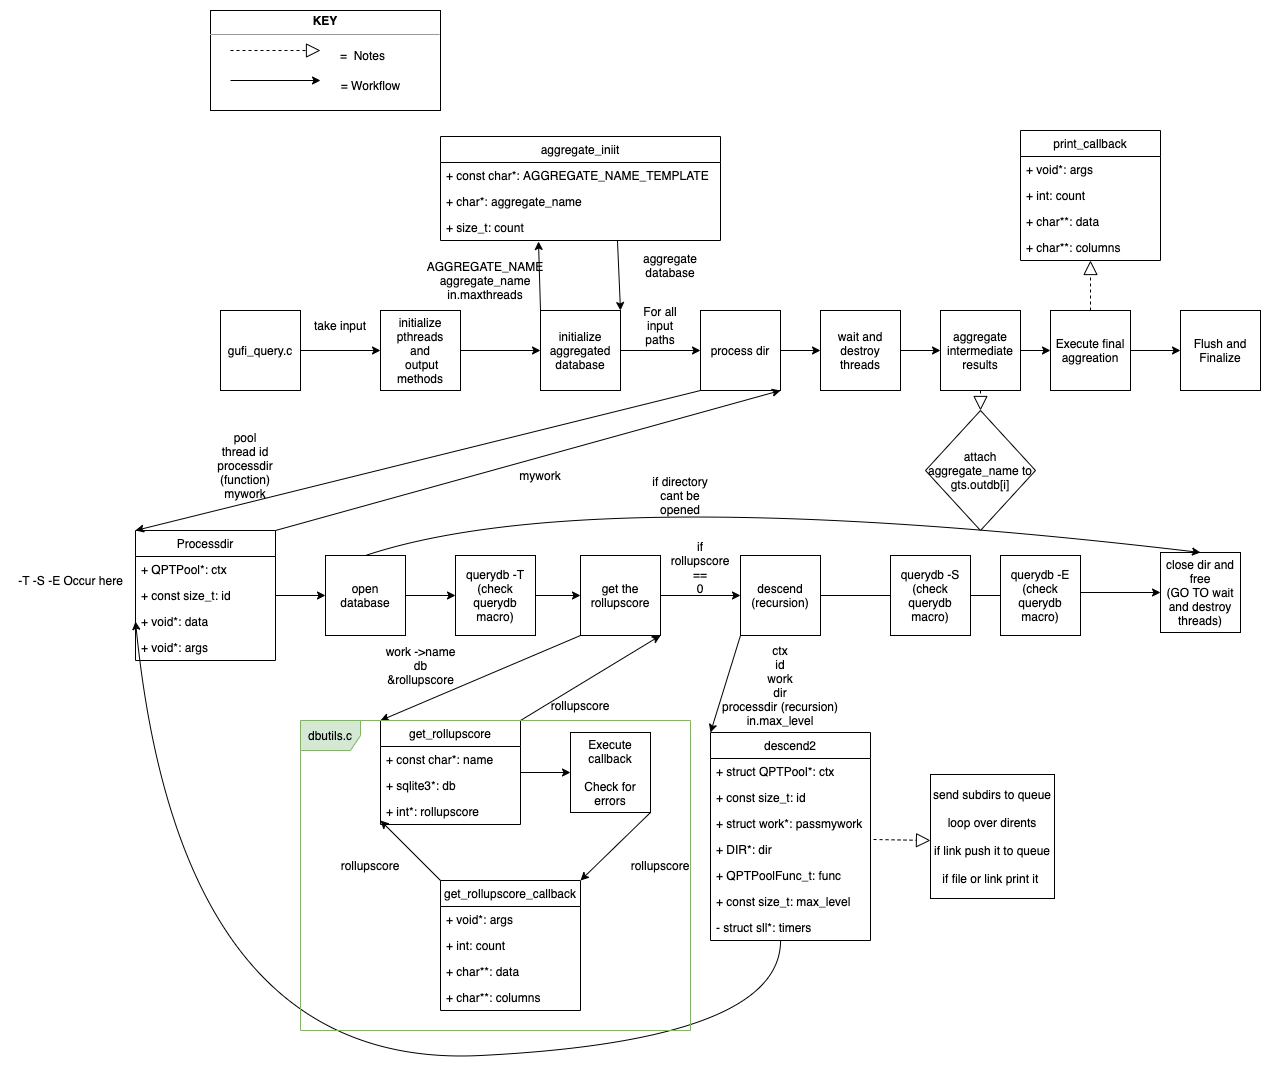
\includegraphics[width=1.0\textwidth]{images/gufi_query.png}
\caption{\label{fig:gufi_query}Workflow of gufi\_query}
\end{figure}
